% UC Davis poster built from the Gemini theme
% (https://github.com/anishathalye/gemini) and inspired by
% Rylan Schaeffer's Stanford template
% (https://github.com/RylanSchaeffer/Stanford-LaTeX-Poster-Template).
%
% COMPILE WITH XeLaTeX (Overleaf: Menu > Settings > Compiler > XeLaTeX).
% The Gemini theme uses fontspec, which requires XeLaTeX or LuaLaTeX.

\documentclass[final]{beamer}

% ====================
% Packages
% ====================

\usepackage[T1]{fontenc}
\usepackage{lmodern}
\usepackage[size=custom,width=120,height=72,scale=1.0]{beamerposter}
\usetheme{gemini}
\usecolortheme{ucdavis}
\usepackage{graphicx}
\usepackage{booktabs}
\usepackage{tikz}
\usepackage{pgfplots}
\usepackage[most]{tcolorbox}
\pgfplotsset{compat=1.17}

% ====================
% Lengths — 4 equal columns
% ====================

\newlength{\sepwidth}
\newlength{\colwidth}
\setlength{\sepwidth}{0.02\paperwidth}
\setlength{\colwidth}{0.22\paperwidth}

\newcommand{\separatorcolumn}{\begin{column}{\sepwidth}\end{column}}

% ====================
% Title / authors
% ====================

\title{Risk Estimation of Preeclampsia}

\author{Ahmed Khan \and Lawrencedel Legaspi \and Selena Phu}

\institute[shortinst]{Department of Electrical and Computer Engineering}

% ====================
% Footer
% ====================

\footercontent{%
  \rlap{\href{https://github.com/AhmedKhan-GH/repnet}{github.com/AhmedKhan-GH/repnet}}%
  \hfill
  UC Davis Senior Design Showcase 2026%
  \hfill
  \llap{\href{mailto:aekhan@ucdavis.edu}{aekhan@ucdavis.edu} | \href{mailto:lawlegaspi@ucdavis.edu}{lawlegaspi@ucdavis.edu} | \href{mailto:slphu@ucdavis.edu}{slphu@ucdavis.edu}}}

% ====================
% Logos: UC Davis ECE logo (left), RUbiNet project logo (right)
% ====================

\logoleft{
\includegraphics[height=9cm]{logo.png}}
\logoright{
\includegraphics[height=5.5cm]{ece_header_white_text.png}}

% ====================
% Body
% ====================

\begin{document}

\begin{frame}[t]
\begin{tikzpicture}[remember picture, overlay]
  \node[anchor=north east, font=\fontsize{100}{100}\selectfont\bfseries,
        text=white, fill=white, rounded corners=8pt, inner sep=10pt,
        text=black] at ([xshift=-3cm, yshift=-2cm]current page.north east) {117};
\end{tikzpicture}
\begin{columns}[t]
\separatorcolumn

% =========================================================
% Column 1 — Introduction & Methods
% =========================================================
\begin{column}{\colwidth}

  \begin{block}{Introduction}

    Preeclampsia is a hypertensive disorder of pregnancy that can occur after 20 weeks of
    gestation~\cite{mayoclinic_preeclampsia}. It can cause complications including
    liver damage, low platelet count, and preterm birth. The disorder can worsen to eclampsia, affecting brain
    function and putting the mother at risk of comas and seizures.
    Delivery is the only definitive treatment, so it is
    imperative to predict a mother's risk of preeclampsia so preventive
    measures can be taken to ensure the health of the mother and the
    fetus. We use different methods of machine learning on 12-lead ECGs
    to estimate risk.

    We present RepNet, a pair of machine-learning models for risk
    estimation of preeclampsia from 12-lead ECGs. RepNet-SE is a
    lightweight CNN (65,748 parameters) with multi-scale
    depthwise-separable convolutions, squeeze-and-excitation, and
    cross-lead self-attention. RepNet-RF is a decision-tree ensemble
    trained on hand-engineered features extracted via NeuroKit2 and GE
    MUSE-reported measurements.

  \end{block}

  \begin{block}{Prior Work}

    Preeclampsia induces measurable cardiac changes: Raffaelli et al.\
    documented altered ventricular repolarization and QT
    dispersion~\cite{raffaelli2014repolarization}, Angeli et al.\ linked
    left atrial ECG abnormalities to a fourfold increased risk of
    hypertensive disorders~\cite{angeli2015ecg}, and a recent
    meta-analysis found preeclampsia prolongs QTc by 21.7\,ms beyond
    normal third-trimester values~\cite{aboshady2025qtc}. Butler et al.\
    showed a ResNet CNN can detect preeclampsia from raw ECG
    waveforms~\cite{butler2024preeclampsia}.

  \end{block}

  \begin{block}{Dataset Analysis}

    2,178 clinical 12-lead ECGs (335 PreE+, 15.4\%) from 1,383
    patients at UC Davis Health. 403 at 250\,Hz natively; 1,788
    at 500\,Hz decimated to 250\,Hz ($q{=}2$, Chebyshev I
    anti-aliasing). Class ratio 5.5:1.

    Power spectral density peaks at 1.0\,Hz, indicating
    low-frequency morphological differences. Silhouette score of
    0.015 confirms classes are inseparable by simple statistics.
    Frobenius norm of the inter-lead correlation difference
    $\|\mathbf{C}_{\mathrm{PE}} - \mathbf{C}_{\mathrm{N}}\|_F = 1.026$
    --- lead coupling preserved in preeclampsia, motivating
    per-lead weight sharing to multiply effective training samples
    by 12$\times$.
    $\mathrm{CV}_{-\log_{10}(p)} = 2.236$ --- unequal lead
    significance, motivating cross-lead self-attention.

  \end{block}

  \begin{block}{RepNet-SE: Neural Network Methods}

    RepNet-SE is a lightweight CNN (65,748 parameters) with three
    stages of multi-scale depthwise-separable convolutions,
    squeeze-and-excitation blocks, and 4-head cross-lead
    multi-head attention, fused via per-lead global average pooling
    and a lead-attention gate.

    Preprocessing applies baseline wander removal, 60\,Hz notch
    filtering, and per-lead z-score normalization. Training uses
    5-model bagging with patient-grouped stratified splits, Adam
    optimizer, class-weighted cross-entropy, and AUROC-based early
    stopping. Evaluation spans 20 seeds with 80/20 splits.

  \end{block}

\end{column}

\separatorcolumn

% =========================================================
% Column 2 — RepNet-SE Methods & Interpretability
% =========================================================
\begin{column}{\colwidth}

  \begin{block}{RepNet-SE: Neural Network Results}

    \begin{figure}
      \centering
      
\includegraphics[width=0.95\colwidth]{../final_report/figures/roc_pr_curves.png}
    \end{figure}
    \vspace{-1em}
    \begin{figure}
      \centering
      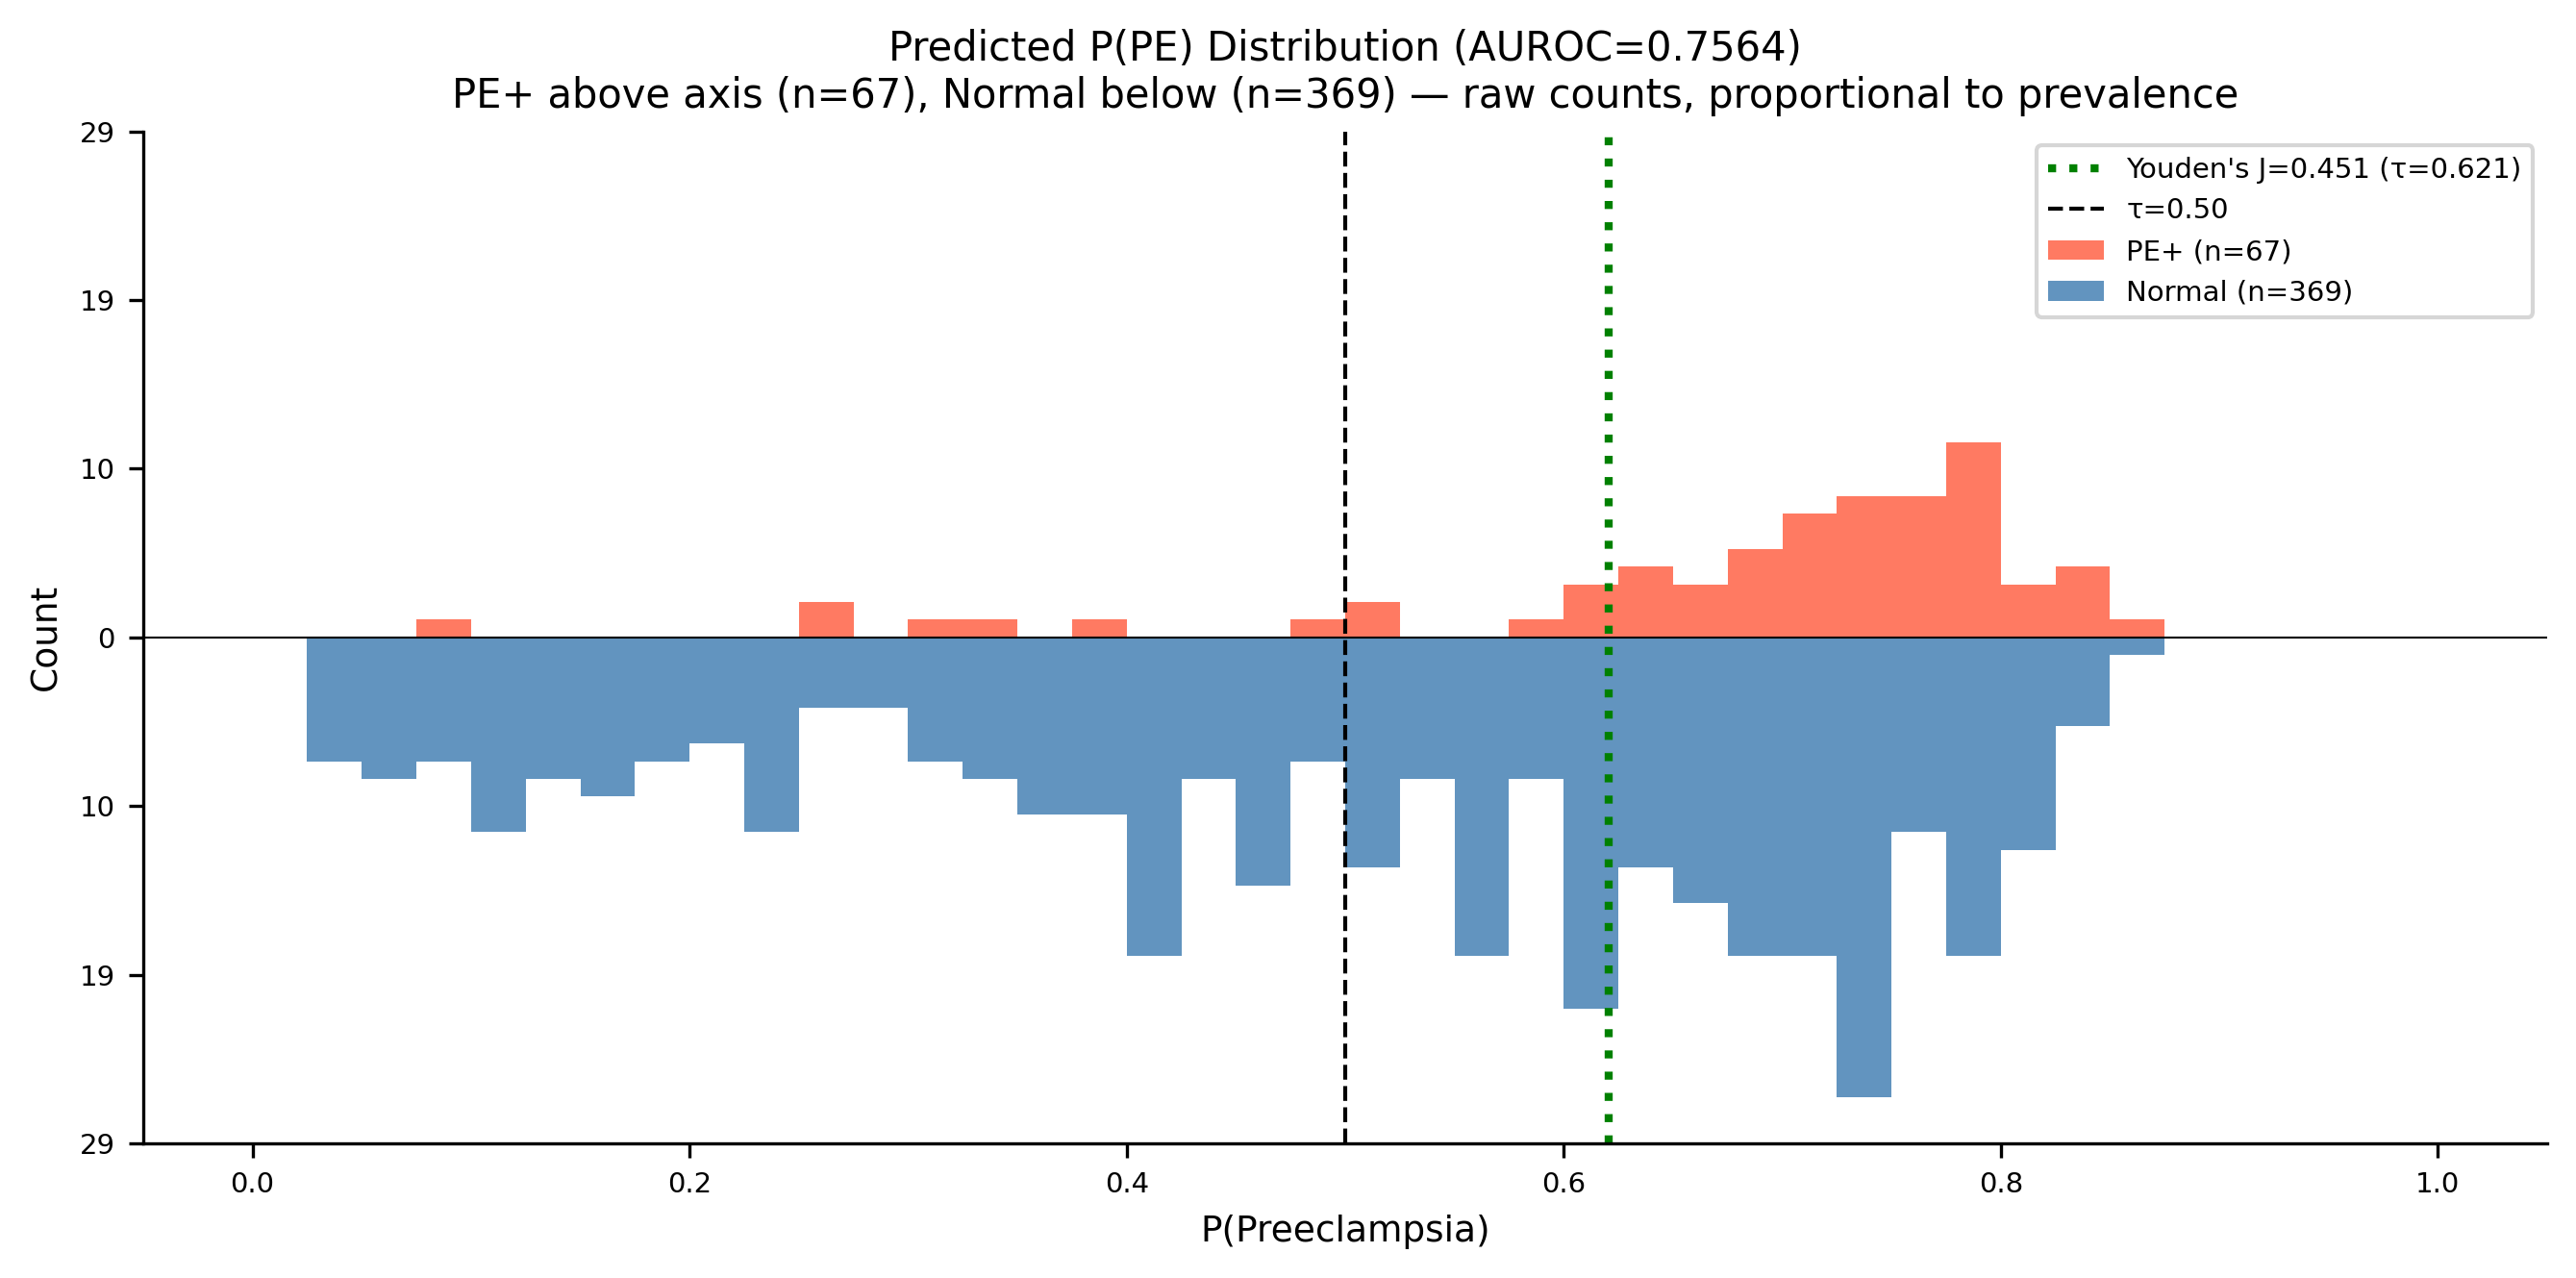
\includegraphics[width=0.95\colwidth]{../final_report/figures/pred_histogram.png}
    \end{figure}

    RepNet-SE achieves a best AUROC of 0.787, AUPRC of 0.362,
    and Brier score of 0.275. The predicted probability
    distribution shows clear rightward shift for preeclamptic
    cases, with Youden's optimal threshold at $\tau = 0.621$.

  \end{block}

  \begin{block}{RepNet-SE: Model Interpretability}

    \begin{figure}
      \centering
      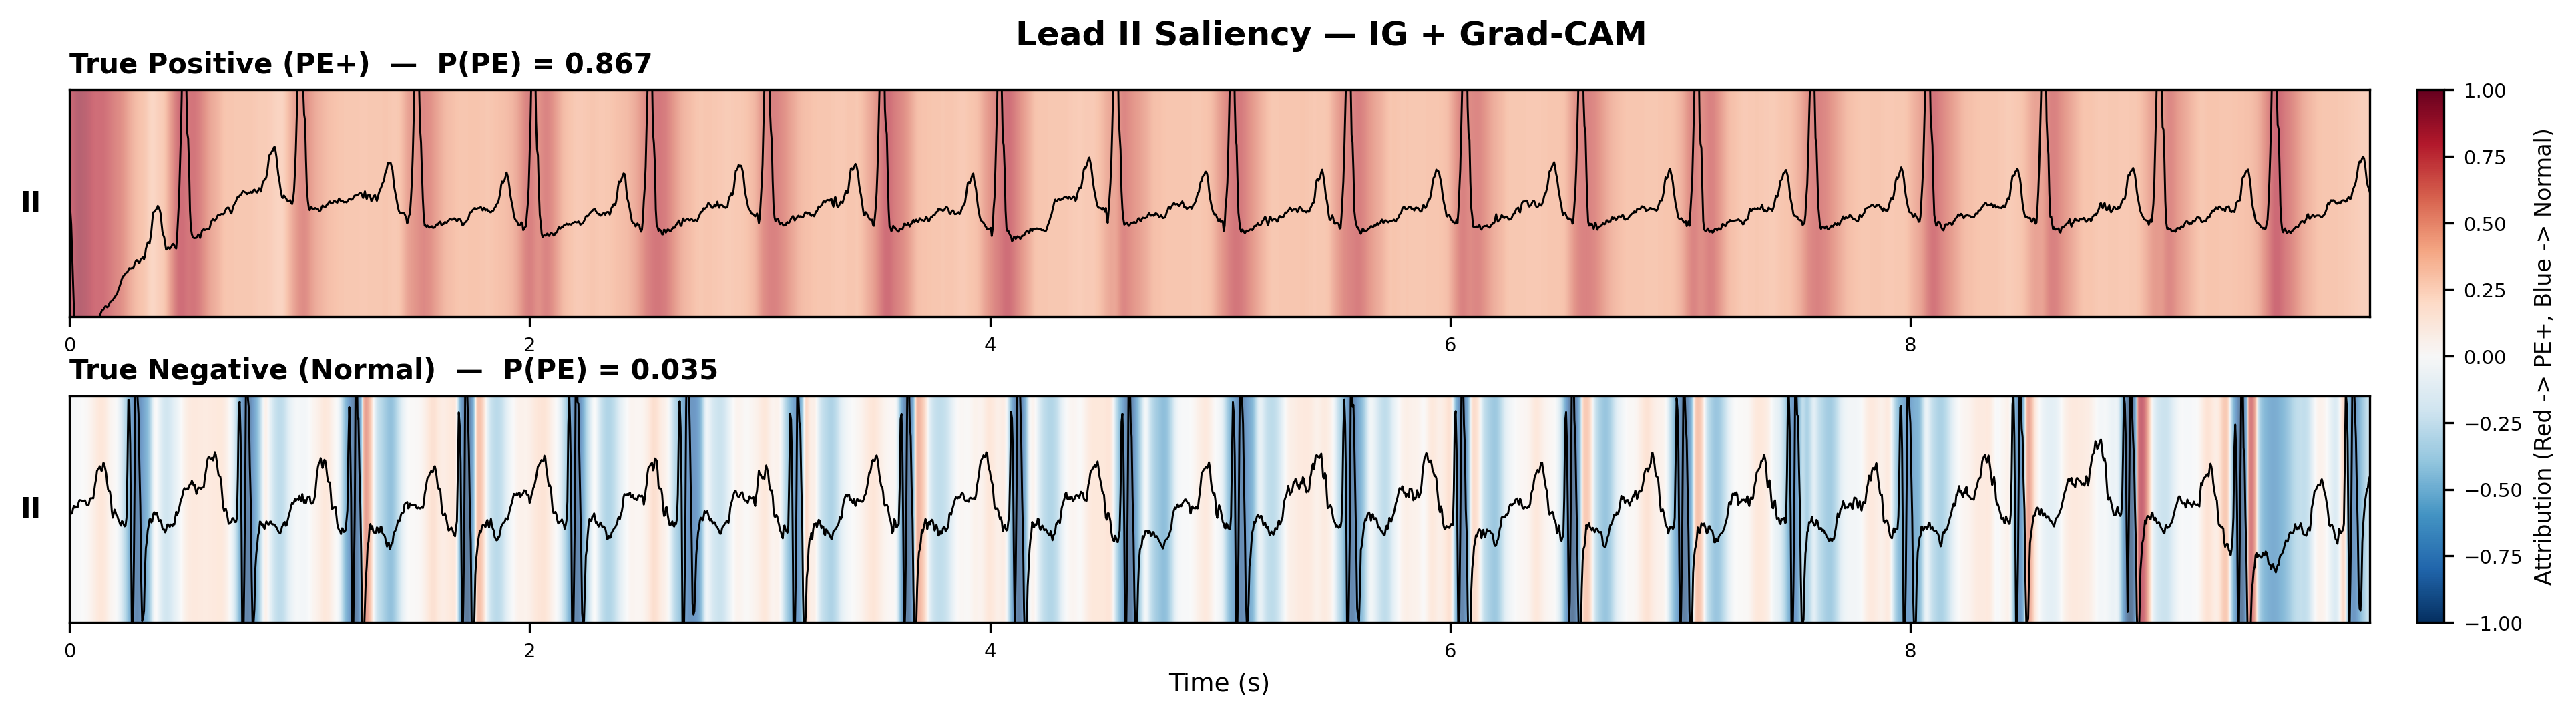
\includegraphics[width=0.95\colwidth]{../final_report/figures/saliency_poster_lead_II.png}
    \end{figure}
    \vspace{-1em}
    \begin{figure}
      \centering
      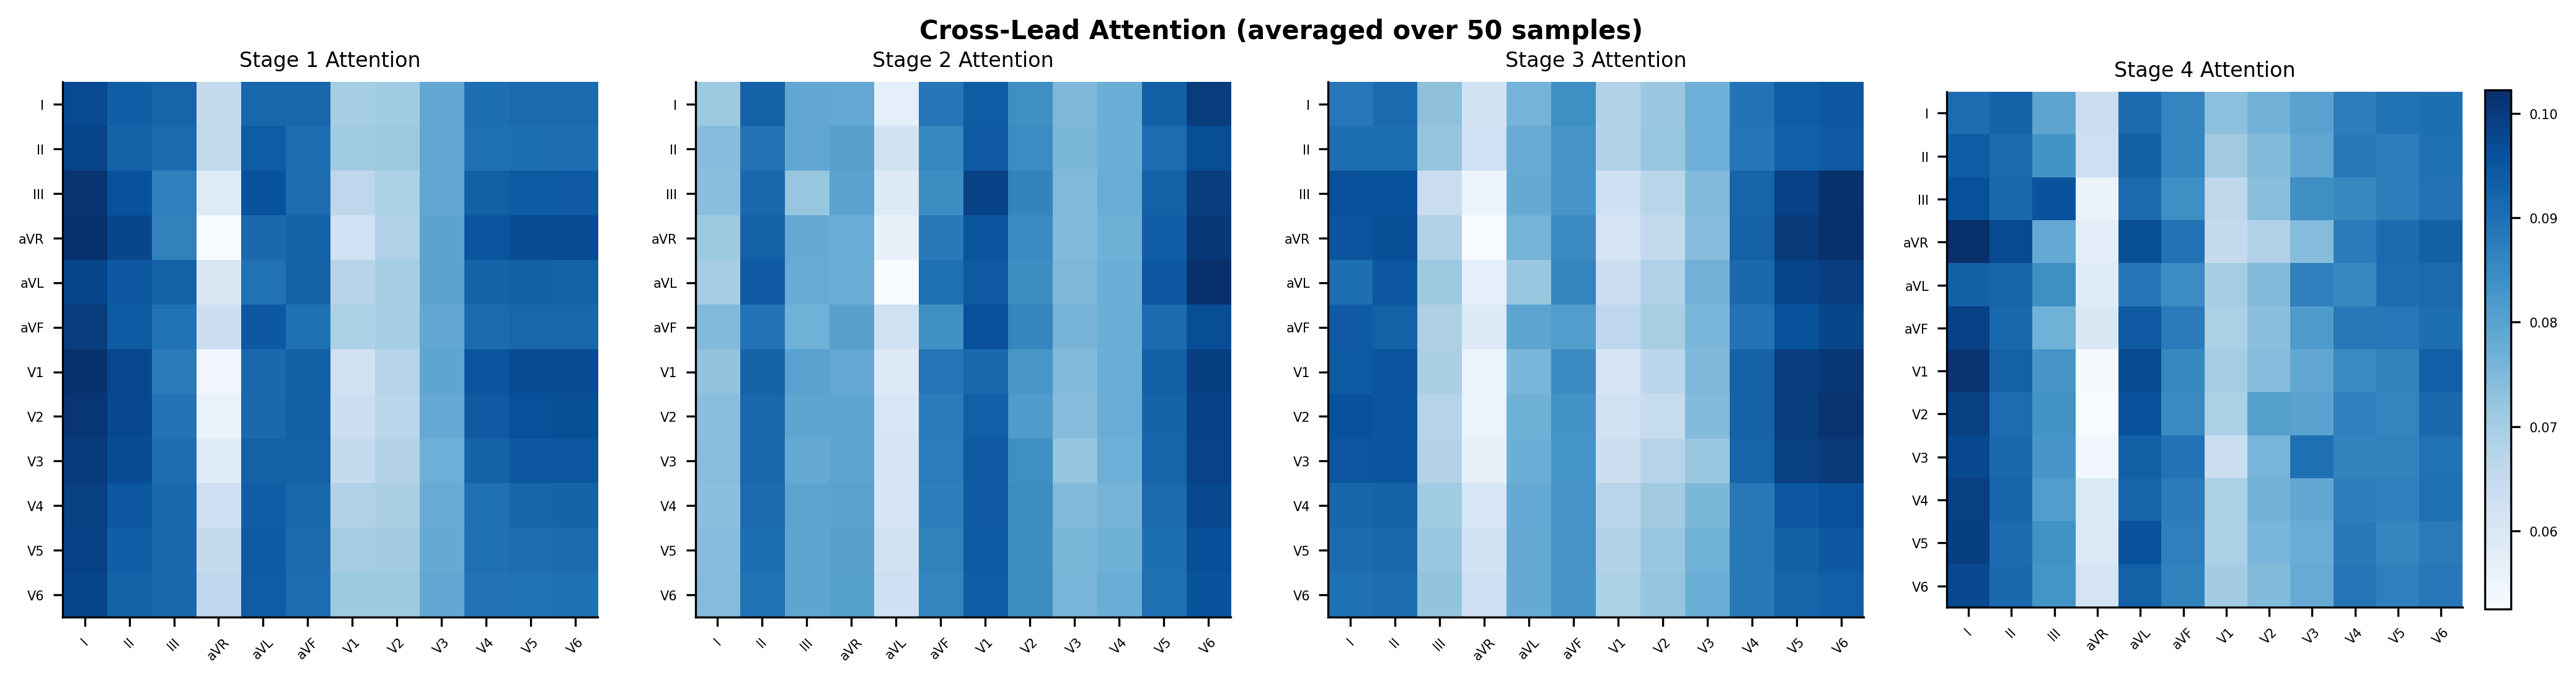
\includegraphics[width=0.95\colwidth]{../final_report/figures/crosslead_attention_stages.png}
    \end{figure}

    Grad-CAM saliency on Lead II highlights QRS and ST-segment
    regions for true positives, confirming the model focuses on
    clinically relevant morphology. Cross-lead attention shows
    increasing specialization across stages, with lateral and
    inferior leads receiving stronger weight. Vertical stripes
    indicate all query leads attend to the same informative keys.

  \end{block}

\end{column}

\separatorcolumn

% =========================================================
% Column 3 — RepNet-RF
% =========================================================
\begin{column}{\colwidth}

  \begin{block}{RepNet-RF: Decision-Tree Methods}

    \begin{enumerate}
      \item Preprocess ECG data using NeuroKit2 to extract features
      \item Add extracted NeuroKit2 features to the MUSE-reported dataset
      \item Apply feature importance methods:
        Pearson Correlation, ANOVA, RFE
      \item Train decision-tree models with ensemble methods
    \end{enumerate}

    Original modeling used a Random Forest with 5-fold
    StratifiedGroupKFold and RandomUnderSampler. Further ensemble
    methods were tested to improve performance.

    \vspace{-0.5em}
    \begin{figure}
      \centering
      \resizebox{\colwidth}{!}{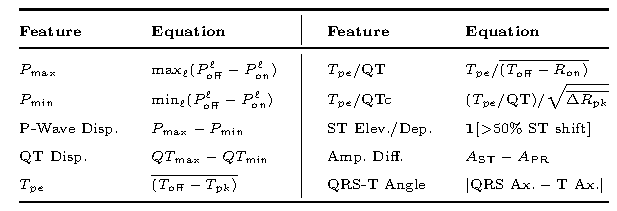
\includegraphics{neurokit_table.pdf}}
      \vspace{-1em}
      \caption{NeuroKit2-derived features (per lead).}
    \end{figure}
    \vspace{-1.5em}

  \end{block}

  \begin{block}{RepNet-RF: Decision-Tree Results}

    Unweighted Voting with SVM and Logistic Regression proved best
    when focusing on sensitivity and balanced accuracy --- metrics that
    reveal how well the model identifies preeclamptic ECGs and genuinely
    distinguishes between classes.

    \begin{table}
      \centering
      \footnotesize
      \resizebox{0.95\colwidth}{!}{%
      \begin{tabular}{l c c c c c}
        \toprule
        \textbf{Ensemble} & \textbf{AUROC} & \textbf{AUPRC} & \textbf{Sens.} & \textbf{Bal.\ Acc.} & \textbf{F1} \\
        \midrule
        Unweighted Voting & 74.54$\pm$4.16 & 41.81$\pm$7.86 & 59.32$\pm$10.70 & 66.79$\pm$3.60 & 38.94 \\
        Weighted Voting & 74.75$\pm$4.48 & 42.26$\pm$7.92 & 60.23$\pm$10.88 & 67.49$\pm$3.45 & 39.80 \\
        \textbf{Unwtd.\ + SVM/LR} & \textbf{75.72$\pm$3.94} & 41.58$\pm$8.03 & \textbf{62.35$\pm$10.93} & \textbf{68.50$\pm$3.22} & \textbf{40.85} \\
        Stacking & 74.77$\pm$4.35 & \textbf{42.43$\pm$7.59} & 59.62$\pm$10.80 & 67.00$\pm$3.46 & 39.17 \\
        Bagging CatBoost & 74.81$\pm$4.98 & 41.96$\pm$8.86 & 59.62$\pm$15.19 & 67.16$\pm$5.59 & 39.10 \\
        \bottomrule
      \end{tabular}%
      }
      \caption{Performance of tree-based ensemble methods on the UCDH dataset.}
    \end{table}

    To identify the most robust cardiological markers and eliminate noisy
    variables, we evaluated our feature space across multiple selection
    methods: Pearson Correlation, ANOVA, and RFE (scoring on balanced
    accuracy, AUROC, and average precision).

    \begin{figure}
      \centering
      
\includegraphics[width=0.95\colwidth]{Heatmap12leads.png}
      \caption{Feature selection consensus heatmap across 12 ECG leads.}
    \end{figure}

    The horizontal distribution illustrates consensus across feature importance
    scores, where darker blocks reveal important features for the
    lead. Global features are not reported here.

  \end{block}

\end{column}

\separatorcolumn

% =========================================================
% Column 4 — Future Work, Acknowledgements, References
% =========================================================
\begin{column}{\colwidth}

  \begin{block}{Conclusion}

    RepNet-SE achieves a best AUROC of 0.787 and RepNet-RF
    achieves 0.757, demonstrating that 12-lead ECGs contain
    discriminative signal for preeclampsia risk estimation
    despite 5.5:1 class imbalance. Both models independently
    converge on clinically relevant markers --- QRS
    morphology, ST-segment changes, $T_{pe}$ interval ---
    consistent with known cardiac effects of preeclampsia.
    Grad-CAM saliency and cross-lead attention confirm the
    neural network learns these patterns without explicit
    feature engineering. Broad ECG-based screening can
    enable early risk estimation of preeclampsia and
    improve maternal and fetal outcomes.

  \end{block}

  \begin{block}{Future Work}

    \begin{itemize}
      \item \textbf{Lead Reduction \& Wearables:} Reduced lead
        sets (e.g.\ leads I, II, V2, V4) or single-lead models
        could enable screening via smart wearables such as
        Apple Watch ECGs.
      \item \textbf{Transfer Learning:} Pretraining on large
        public ECG corpora (PTB-XL, MIMIC-IV-ECG) or
        leveraging ECG foundation models before fine-tuning on
        the UCDH cohort.
      \item \textbf{Multi-Site Validation:} Current results are
        from a single site; external validation on diverse
        populations is needed to assess generalizability.
      \item \textbf{Demographic Integration:} Incorporating
        maternal age, gestational age, and clinical history
        as auxiliary inputs alongside ECG data.
      \item \textbf{Feature Importance Across Models:} Feature
        selection used Random Forest; models such as CatBoost
        or LightGBM may retain different useful features.
    \end{itemize}

  \end{block}

  \begin{block}{Acknowledgements}
    Dr.\ Lihong Mo, MD, PhD (OB/GYN);
    Dr.\ Chen-Nee Chuah, PhD (EECS).

    \textbf{Graduate Mentors:} Hana Shaik, Arielle Yoo.

  \end{block}

  \vfill

  \begin{block}{References}

    \begin{tcolorbox}[boxrule=0.5pt, colback=white, colframe=black, arc=2pt]
    \tiny{\bibliographystyle{plain}\bibliography{poster}}
    \end{tcolorbox}

  \end{block}

\end{column}

\separatorcolumn
\end{columns}
\end{frame}

\end{document}
